\chapter{Introducción}\label{cap.introduccion}
En este capítulo se definirá el contexto en el cual se sitúa este proyecto así como la motivación principal que ha llevado a desarrollarlo. Se explicará de forma general qué es la robótica, sus aplicaciones y algunas piezas software utilizado para la programación de robots. También se expondrá su uso en docencia hoy en día y se comentará de manera general la plataforma JdeRobot-Academy en la que se encuadra este Trabajo Fin de Grado (TFG).

\section{Robótica}
La robótica es una rama de la ingeniería que emplea la informática para diseñar y desarrollar sistemas que permitan facilitar la vida del ser humano, e incluso sustituirle en determinadas tareas. Esta rama usa conceptos de diversas disciplinas, tales como la física, las matemáticas, la electrónica, la mecánica, la inteligencia artificial o la ingeniería de control. Mediante todas estas disciplinas crea diversas máquinas que ejecutan diferentes comportamientos en función de su propósito. Estas máquinas se denominan ``robots''. En el futuro, dominar esta disciplina será clave debido a que cada vez de forma más habitual se implantan robots en diferentes empleos. \\

Los robots pueden tener formas variadas. Según su arquitectura física los robots pueden ser:

\begin{itemize} 
    	\item Brazos robotizados: Son robots de base fija, aunque en algunas ocasiones pueden realizar desplazamientos limitados, y mover sus extremidades en un espacio de trabajo concreto mediante algún sistema de coordenadas y con un limitado número de grados de libertad. Pueden ser muy diferentes en su forma y configuración. Se emplean habitualmente en zonas de trabajo amplias o alargadas. Los robots industriales, manipuladores y cartesianos son algunos ejemplos.
    	
		\item Robots móviles: Tienen una importante capacidad de movimiento. Son capaces de realizar un cierto desplazamiento, mediante la información que les proporcionan sus sensores del entorno o mediante tele-mando. Suelen tener un sistema locomotor de tipo rodante. Estos robots son capaces de evitar obstáculos y tienen un nivel de inteligencia considerablemente alto. Se suelen emplear para transportar piezas en una cadena de fabricación.
		
		\item Humanoides: Estos robots intentan imitar de manera parcial o total la forma y el comportamiento del movimiento humano. 
		
		\item Zoomórficos: La principal característica de estos robots es su sistema de locomoción, el cual pretende imitar a los distintos seres vivos.
\end{itemize}


\subsection{Aplicaciones de la robótica}
Actualmente la robótica está en continua expansión. Se pueden encontrar robots en diferentes áreas y entornos. Una de las principales áreas donde se encuentran robots es en la industria. Gracias a los robots se pueden abordar tareas peligrosas y complejas. El robot industrial, debido a su naturaleza multifuncional, puede llevar a cabo un gran número de tareas, totalmente inalcanzable si la mano de obra es humana, de manera que se abarata mucho el coste de producción. \\

En el mundo del automóvil se han introducido robots tanto para su construcción, utilizando brazos mecánicos en las cadenas de montaje, como para lograr que los coches sean autónomos. Una de las empresas pioneras en este ámbito es Google que junto con Fiat-Chrysler han desarrollado el proyecto ``Waymo'' (Figura~\ref{fig.coches}). Estos vehículos autónomos tienen sensores y software diseñado para detectar personas, ciclistas, vehículos, ciclistas y carreteras a una distancia mayor que dos campos de fútbol en todas las direcciones. \\

La empresa Tesla también ha desarrollado coches autónomos (Figura~\ref{fig.coches}). Sus coches tienen instaladas ocho cámaras que ofrecen una visión de 360 grados alrededor del vehículo en un área de hasta 250 metros. Además, dispone de doce sensores ultrasónicos capaces de detectar objetos de todo tipo y tamaño alrededor del coche, y de un radar delantero que ofrece datos adicionales.\\

El objetivo de los coches autónomos es evitar los accidentes de tráfico y disminuir los atascos. \\

\begin{figure}[H]
  \begin{center}
    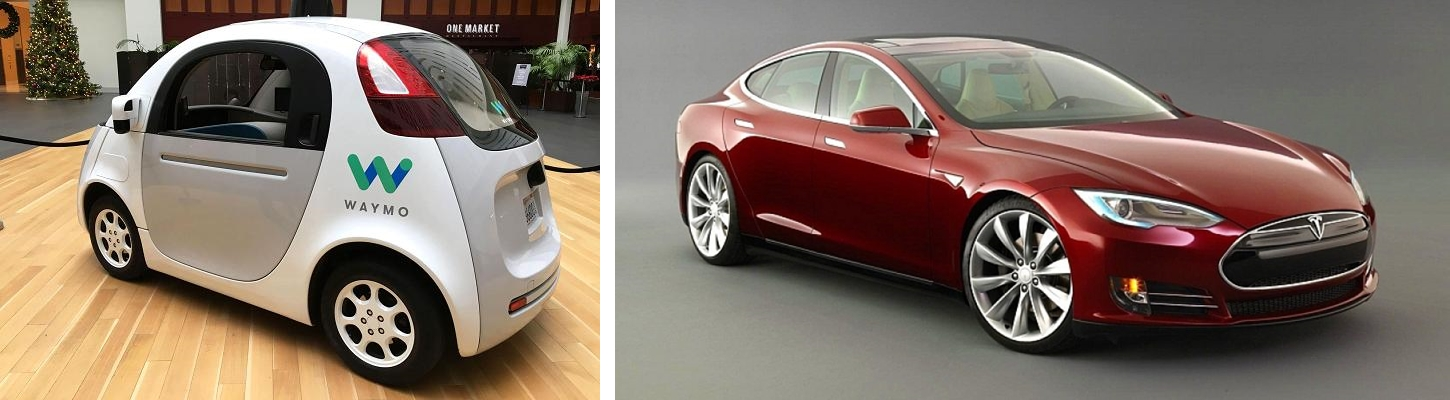
\includegraphics[width=0.8\textwidth]{figures/Introduccion/coches.jpg}
		\caption{Coches autónomos Waymo y Tesla}
		\label{fig.coches}
		\end{center}
\end{figure}

También se pueden encontrar robots en los hogares de las personas, como por ejemplo aspiradoras autónomas. Estas aspiradoras mediante sensores y el desarrollo de tecnologías robóticas como la construcción de mapas y los sistemas de navegación son capaces de limpiar las casas de una manera fiable y robusta ante distintos tipos de obstáculos como muebles o escaleras. La empresa iRobot es pionera mundial en este sector con su aspiradora Roomba, aunque también se pueden encontrar otras aspiradoras potentes en el mercado como el robot aspirador Dyson (Figura~\ref{fig.dyson_amazon}) que calcula un patrón de modo sistemático y de esa forma sabe por dónde ha pasado y dónde tiene que ir a limpiar.\\

Amazon, en sus almacenes, también ha introducido robots para que la logística sea mucho más rápida y eficaz (Figura~\ref{fig.dyson_amazon}). Utiliza la automatización para almacenar y retirar los productos. Sus robots son capaces de cargar hasta 1300 Kg y mediante el uso de un láser y una cámara en la parte delantera, son capaces de detectar obstáculos. Se mueven a 1,7 metros por segundo y satisfacen un pedido en 15 minutos en vez de en 70, disminuyendo así el tiempo de entrega de sus productos.

\begin{figure}[H]
  \begin{center}
    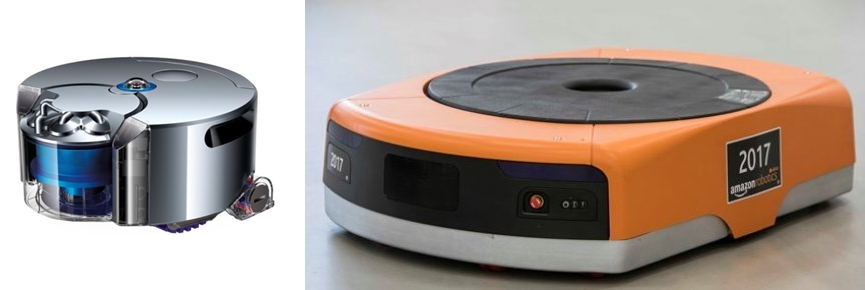
\includegraphics[width=0.8\textwidth]{figures/Introduccion/dyson_amazon.jpg}
		\caption{Robot aspirador Dyson y robot de Amazon Drive}
		\label{fig.dyson_amazon}
		\end{center}
\end{figure}

También se pueden encontrar robots en otra gran variedad de ámbitos:
	
\begin{itemize}
		\item Robots médicos: La aplicación fundamental de estos robots se sitúa en el campo de la cirugía. Es fundamental que los diversos brazos robóticos que se emplean en alguna operación quirúrgica sean lo suficientemente precisos. Pueden ser controlados a distancia. 
		
		\item Robots industriales: Son robots automáticos, reprogramables y con múltiples funciones. Poseen tres o más ejes para poder orientar y colocar en la posición correcta diferentes piezas, materiales, dispositivos o herramientas. Son empleados en la realización de diferentes tareas de la producción industrial en sus diversas etapas. Su entorno de trabajo suele estar controlado, esto hace que las funciones de los robots se simplifiquen de manera notable. 
		
		\item Robots militares: Estos robots tienen aplicaciones militares concretas, para las cuales pueden actuar de forma autónoma o estar controlados de forma remota. Presentan diferentes morfologías en función de su uso. Asisten o guían al ejército en operaciones especiales. Sus funciones pueden ser la búsqueda, el transporte, el rescate o el ataque.
		
		\item Robots educativos: Estos robots se crearon con el fin de emplearse en la enseñanza, especialmente en escuelas e institutos. Los robots educativos de LEGO Mindstorms son un buen ejemplo.
		
		\item Robots de servicio: De forma habitual, se emplean para reemplazar al ser humano en entornos no controlados, hostiles y donde puede ser necesario un cambio de forma del robot. Son dispositivos electromecánicos controlados por ordenador y normalmente dotados de movimiento. Suelen poseer uno o varios brazos mecánicos independientes. No realizan tareas industriales.
		
		\item Robots de investigación: son empleados habitualmente en los laboratorios de las Universidades. Están destinados a la investigación y por ello pueden ser de muy diversas formas. Pueden tener un fin concreto en algún proyecto de investigación o no tener ninguna aplicación concreta.
	\end{itemize}


\section{Software para robots}
Además del hardware, el otro ingrediente fundamental de los sistemas robóticos es su software. Mediante el software se le indica al robot las acciones que tiene que realizar, dotándole así de inteligencia y autonomía. Este desarrollo de software suele ser complicado y arduo. En la actualidad, se han propuesto muchos entornos (middleware) y bibliotecas para hacer más fácil la programación de los robots. 

\subsection{Middleware}
Los robots autónomos son sistemas complejos que requieren de la interacción entre numerosos componentes heterogéneos. Debido al aumento de la complejidad de las aplicaciones robóticas y la diversa gama de hardware, el middleware robótico está diseñado para gestionar la complejidad y la variedad del hardware y las aplicaciones. Permiten a una aplicación interactuar o comunicarse con otras aplicaciones, sistemas operativos, redes o dispositivos. Los middlewares robóticos proporcionan una API (Interfaz de Programación de Aplicaciones) que simplifica la comunicación entre las aplicaciones robóticas y el hardware subyacente (como los sensores y actuadores), simplificando así el diseño del software y mejorando su calidad. \\

El middleware más extendido, y que se ha convertido en un estandard de facto es ROS (Robot Operating System) \footnote{\url{http://www.ros.org/}}. Es un entorno de programación de código abierto mantenido por la Open Source Robotics Foundation (OSRF). Ofrece una colección de herramientas, bibliotecas y convenciones que tienen como objetivo simplificar la tarea de crear un comportamiento robótico complejo y robusto en una amplia variedad de plataformas robóticas. Está orientado a sistema UNIX (Ubuntu (Linux)), aunque también se está adaptando a otros sistemas operativos como Fedora, MacOS-X, Arch, Gentoo, OpenSUSE, Slackware, Debian o Microsoft Windows, considerados como ``experimentales''.\\

Existen otros middleware como Orca, JdeRobot, Player-Stage, Orocos, etc. pero su ámbito de utilización es más reducido
que el de ROS.
	

\subsection{Bibliotecas}
En informática, una biblioteca es un conjunto de funciones, codificadas en un lenguaje de programación, que ofrece una interfaz bien definida para la funcionalidad que se invoca. Su fin es ser utilizada por otros programas. \\

Una de las bibliotecas de visión artificial utilizadas en robótica es OpenCV \footnote{\url{http://opencv.org/}}. Contiene más de quinientas funciones que abarcan una gran gama de áreas en el proceso de visión, como reconocimiento de objetos y reconocimiento facial. Otro ejemplo es PLC \footnote{\url{http://pointclouds.org/}}. Se utiliza para el procesamiento digital de imágenes mediante el tratamiento de nubes de puntos aleatorios. Contiene numerosos algoritmos de última generación que incluyen filtrado, estimación de características, reconstrucción de superficies y segmentación entre otros. 

\subsection{Simuladores}
Los simuladores son herramientas muy utilizadas en robótica debido a que, normalmente, los robots suelen ser costosos. Mediante el uso de estos simuladores se consigue hacer todo tipo de pruebas con los robots sin ningún riesgo de dañar o romper el equipo. Estos simuladores representan de manera realista el entorno y los robots, por lo que es recomendable usarlos antes de probar los programas o aplicaciones creados en robots reales. \\

Uno de los simuladores más utilizados es Gazebo \footnote{\url{http://gazebosim.org/}}.Es un simulador 3D de código abierto distribuido bajo licencia Apache 2.0. Accede a múltiples motores de física de alto rendimiento, incluidos ODE \footnote{\url{http://opende.sourceforge.net/}} y Bullet \footnote{\url{http://bulletphysics.org/wordpress/}} entre otros. Al utilizar el motor de renderizado 3D OGRE \footnote{\url{https://www.ogre3d.org/}}, Gazebo proporciona una representación realista de entornos que incluyen iluminación, sombras y texturas de alta calidad. Permite probar rápidamente algoritmos, diseñar robots, simular cámaras, coches y drones, realizar pruebas de regresión y entrenar sistemas de inteligencia artificial utilizando escenarios realistas. Da soporte a Linux, Solaris, * BSD y Mac OSX (Darwin).\\
	
También hay otros simuladores como V-REP, Webots, Stage, etc.. Pero no están tan extendidos como Gazebo.

\section{Robótica en docencia universitaria}

En la docencia universitaria se imparten clases de robótica en los Grados y los Postgrados, en concreto en escuelas de ingeniería. En España, se puede ver la robótica integrada en el ``Grado en Ingeniería Robótica'' de la Universidad de Alicante, y los Grados de ``Electrónica industrial y automática'' o en ``Ingeniería Electrónica, Robótica y Mecatrónica'' en diversas universidades. En los estudios de Postgrado existen Másteres destacados como el ``Máster de Visión Artificial'' en diferentes universidades. En el ámbito internacional se pueden destacar universidades especializadas en robótica como el MIT, Stanford, Georgia Institute of Technology, etc. \\

Cabe destacar como iniciativa privada el entorno de enseñanza robótica TheConstructSim \footnote{\url{http://www.theconstructsim.com/}} cuyo objetivo es enseñar a programar con el middleware ROS.  Contiene una serie de tutoriales ROS en línea vinculados a simulaciones en línea, que brindan las herramientas y el conocimiento necesario para comprender y crear cualquier desarrollo de robótica basado en ROS. Usa robots reales simulados y solo se necesita un navegador web por lo que no requiere instalación.


\subsection{JdeRobot-Academy}
La Universidad Rey Juan Carlos cuenta con el proyecto de software libre en robótica JdeRobot, que incluye el entorno académico JdeRobot-Academy \footnote{\url{https://jderobot.org/JdeRobot-Academy}} \footnote{\url{https://github.com/JdeRobot/Academy}} . Este entorno educativo se ha empleado con éxito en diferentes asignaturas, como son ``Visión en Robótica'' del Máster de Visión Artificial, o ``Robótica'' del Grado de Ingeniería Telemática. Asimismo, la Universidad ofrece cursos de introducción a la robótica y a los drones, empleando dicho entorno. \\

Este TFG se encuadra justo dentro de este entorno JdeRobot-Academy y aborda la creación de dos ejercicios nuevos. Está diseñado para que las prácticas desarrolladas por los alumnos se ejecuten en robots reales y también en simulados sin modificar el código fuente. El lenguaje de programación que se utiliza prácticas es Python debido a su sencillez y la potencia que ofrece. Para ejecutar dichas prácticas en robots, se usa el simulador Gazebo. Este simulador permite aprender robótica aunque no se tengan los robots reales ya que dispone de una gran variedad de robots, como pueden ser drones, coches, aspiradoras o brazos mecánicos, entre otros, pudiendo abarcar distintos aspectos de la robótica. \\

Cada práctica consta de una aplicación académica, que resuelve tareas como la interfaz gráfica (GUI) o la conexión con sensores y actuadores concretos, y que quedan simplificados para el alumno. También contiene el código del estudiante, que simplemente rellena un sencillo fichero plantilla, llamado \texttt{MyAlgorithm.py}, con la lógica del robot, logrando así que se centre solamente en la creación y desarrollo de los algoritmos de percepción, planificación y control habituales en los robots. \\

\begin{figure}[H]
  \begin{center}
    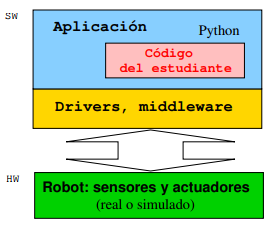
\includegraphics[width=0.4\textwidth]{figures/Introduccion/esquema.png}
		\caption{Diseño de una práctica robótica}
		\label{fig.esquema}
		\end{center}
\end{figure}

En la Figura~\ref{fig.esquema} se puede apreciar cómo está diseñada una práctica en el entorno de JdeRobot-Academy. En la capa inferior se encuentra el robot con sus actuadores (ruedas, motores...) y sensores (láseres, cámaras…) y puede ser tanto simulado como real.  En la capa intermedia se tienen los drivers y middlewares necesarios para la comunicación entre la aplicación y el robot. Y por último, en la capa superior, está la aplicación donde se analizan los datos captados por los sensores y se sitúa el código del estudiante, tomando decisiones de actuación y planificación. \\

En la Figura~\ref{fig.estructura} se puede ver la estructura que tiene cada una de las prácticas y como estan relacionados los distintos componentes.

\begin{figure}[H]
  \begin{center}
    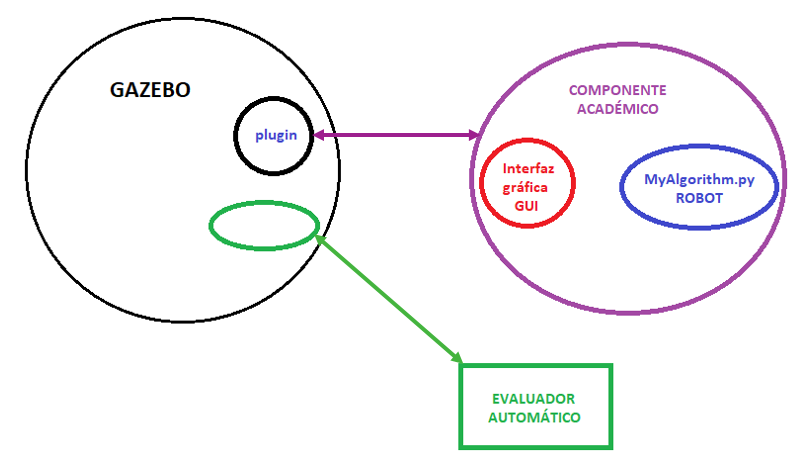
\includegraphics[width=0.9\textwidth]{figures/Introduccion/estructura.png}
		\caption{Estructura de una práctica robótica en JdeRobot-Academy}
		\label{fig.estructura}
		\end{center}
\end{figure}


Los cuatro ámbitos principales en los que actualmente se agrupan los ejercicios disponibles son:

\begin{itemize}
	\item Visión: Aquí se pueden encontrar las prácticas \texttt{Color filter}, cuyo principal objetivo es el uso de filtros de color, y \texttt{Visual 3D reconstruction from a stereo pair of RGB cameras} en la que se reconstruye una escena en 3D a partir de dos cámaras color a bordo de un robot (Figura~\ref{fig.vision}).
	\begin{figure}[H]
  	\begin{center}
    	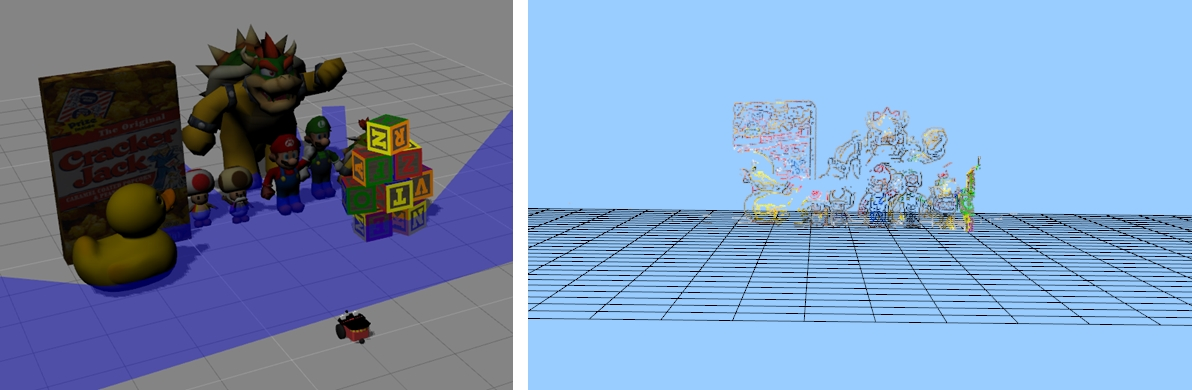
\includegraphics[width=0.9\textwidth]{figures/Introduccion/vision.jpg}
			\caption{Práctica Visual 3D reconstruction}
			\label{fig.vision}
			\end{center}
	\end{figure}

	\item Coches autónomos: En este ámbito se han desarrollado las prácticas \texttt{Visual follow-line behavior on a Formula 1} en la cual los alumnos tienen que conseguir que un coche de Fórmula 1 (Figura~\ref{fig.f1}) logre seguir una línea roja pintada en un circuito de carreras ejercitando para ello el control visual; \texttt{Local navigation of a Formula 1 with VFF}, su objetivo es que el alumno programe un algoritmo de navegación local que consiga que un coche Fórmula 1 recorra un circuito evitando chocar con obstáculos (que son otros coches estacionados a lo largo del circuito); y \texttt{Global navigation of a TeleTaxi with GPP}, en la cual el alumno debe programar un algoritmo de planificación y otro de pilotaje para que un taxi consiga llegar a un punto del mundo en el que se encuentra clicando en una parte del mapa de dicho mundo.
	\begin{figure}[H]
  	\begin{center}
    	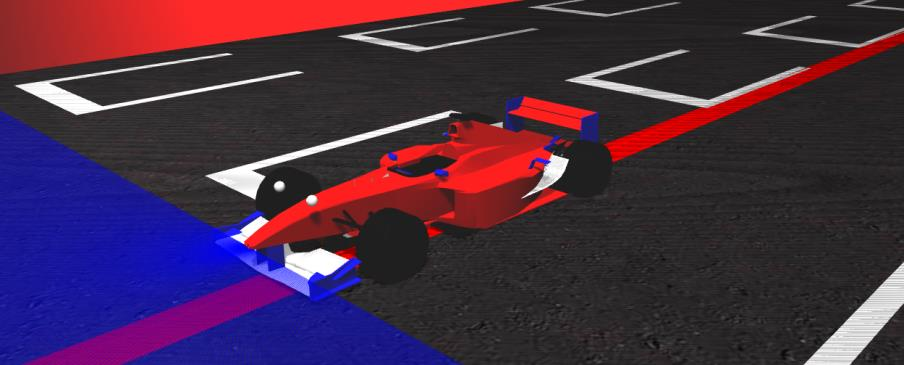
\includegraphics[width=0.5\textwidth]{figures/Introduccion/f1.jpg}
			\caption{Coche de Fórmula 1}
			\label{fig.f1}
			\end{center}
	\end{figure}

	\item Robots móviles: La práctica realizada es  \texttt{Bump and go}, que consiste en programar un autómata finito de estados reactivo con un robot TurtleBot.

	\item Drones: Es el ámbito que posee más prácticas desarrolladas. \texttt{Drone position control navigation} se basa en el uso de controladores PID basados en posición; \texttt{Follow the ground robot}, cuyo objetivo es conseguir que un dron siga a un robot moviéndose en tierra; \texttt{Follow the road}, en la cual, un dron sigue una carretera; \texttt{Drone cat and mouse} que consiste en que un dron juega el papel de gato y tiene que atrapar al dron autónomo que tiene el papel de ratón (Figura~\ref{fig.dron}); \texttt{Landing on a moving car}, en esta práctica hay que lograr que un dron aterrice sobre un coche en movimiento mediante control visual; \texttt{Escaping from a labyrinth using visual clue}, el objetivo es conseguir que un dron salga de un laberinto siguiendo las flechas ubicadas a lo largo de dicho laberinto que se perciben desde visión; y \texttt{People rescue after an earthquake} que consiste en que un dron detecte personas y marque la posición en la que se encuentran.
	
\begin{figure}[H]
  	\begin{center}
    	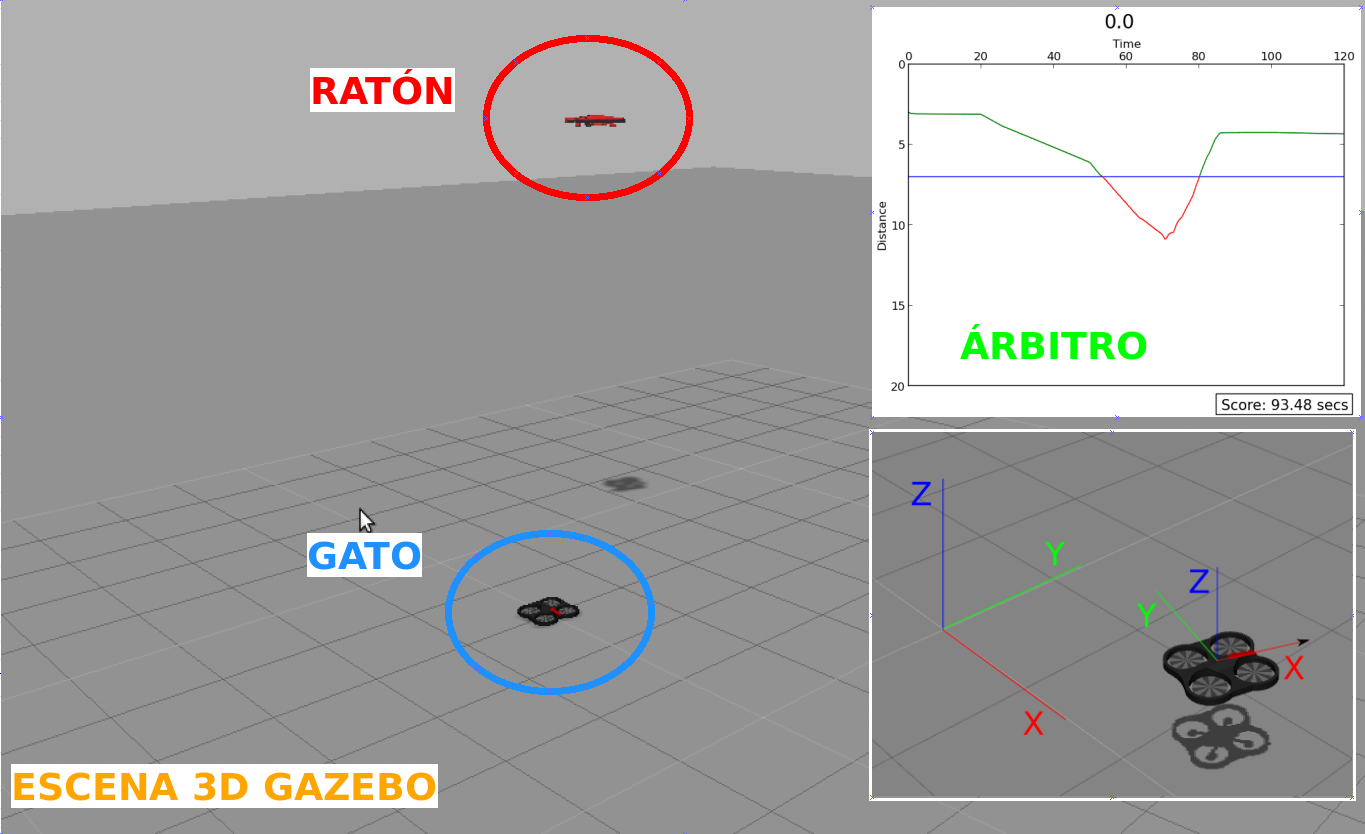
\includegraphics[width=0.8\textwidth]{figures/Introduccion/gatoraton.png}
			\caption{Práctica Drone cat and mouse}
			\label{fig.dron}
			\end{center}
	\end{figure}
\end{itemize}
